\documentclass[t]{beamer}

\usepackage{wrapfig}
\usepackage{float}

% set fonts
\usefonttheme{professionalfonts} % using non standard fonts for beamer
\usepackage{txfonts,mathptmx}

% set indend spacing for first and second level indentation
\setlength{\leftmargini}{0.5cm}
\setlength{\leftmarginii}{0.5cm}

% Set circles for bullets 

\setbeamertemplate{itemize items}[circle]

% increase space between text and frame name
\addtobeamertemplate{frametitle}{}{\vspace{1em}}

%Information to be included in the title page:
\title{Describing Verilog Applications}
\author{Nikola Petrovic}
\institute{University of Belgrade, School of Electrical Engineering}
\date{2022}



\begin{document}

\frame{\titlepage}

%%%%%%%%%%%%%%%%%%%%%%%%%%%%%%%%%%%%%%%%%%%%%%%%%%%%%%%%%%%%
\begin{frame}
\frametitle{Module Objective}

We well explain the nature and use of Hardware Description Language (HDL)
\newline

\textbf{Topics}

\begin{itemize}
\item What the heck is an HDL?
\item levels of abstraction
\item What are the benefits of using HDLs, we do we care?
\item The Verilog HDL
\end{itemize}

\end{frame}


%%%%%%%%%%%%%%%%%%%%%%%%%%%%%%%%%%%%%%%%%%%%%%%%%%%%%%%%%%%%
\begin{frame}
\frametitle{Terms and Definitions}

Hardware Description Language (HDL)
\begin{itemize}
\item A programming-like language that describes the functionality of digital electronic hardware circuits
\end{itemize}
Simulator:
\begin{itemize}
\item Software that imitates the functionality of electronic hardware as described by the HDL
\end{itemize}
Level of Abstraction:
\begin{itemize}
\item The level of detail provided by the utilized modeling style, such as behavioral and gate-level
\end{itemize}
Application Specific Integrated Circuit (ASIC):
\begin{itemize}
\item Integrated circuit developed for specific application
\end{itemize}
\end{frame}

%%%%%%%%%%%%%%%%%%%%%%%%%%%%%%%%%%%%%%%%%%%%%%%%%%%%%%%%%%%%
\begin{frame}
\frametitle{Terms and Definitions Continued}

Bottom-Up Design Flow:
\begin{itemize}
\item A design methodology in which you build the low-level components first and then connect them to make large systems
\end{itemize}
Top-Down Design Flow:
\begin{itemize}
\item A design methodology in which you define the system at the very high level of abstraction and then iteratively refine it
\end{itemize}
Register Transfer Level (RTL):
\begin{itemize}
\item A level of abstraction that defines storage elements and their clocks
\end{itemize}
Tool Command Language (TCL):
\begin{itemize}
\item A scripting language used for issuing commands to interactive programs
\end{itemize}
\end{frame}

%%%%%%%%%%%%%%%%%%%%%%%%%%%%%%%%%%%%%%%%%%%%%%%%%%%%%%%%%%%%
\begin{frame}
\frametitle{What is HDL}

A HDL is a programming language with special constructs for Modeling hardware concurrency and timing.
\newline

A HDL supports design at multiple levels of abstraction:
\begin{wrapfigure}{r}{0.4\textwidth}
  \begin{figure}[H!]
    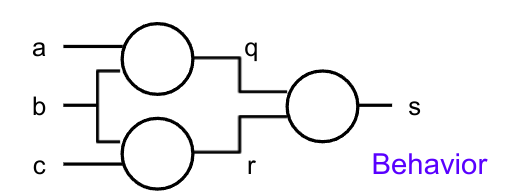
\includegraphics[width=0.38\textwidth]{img/01_beh.png}
    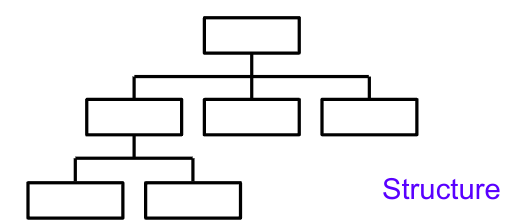
\includegraphics[width=0.38\textwidth]{img/01_struct.png}
    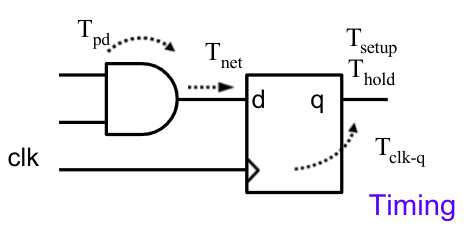
\includegraphics[width=0.38\textwidth]{img/01_tim.png}
  \end{figure}
\end{wrapfigure}
\textcolor{blue}{Behavioral Modeling:}
\begin{itemize}
\item Sequential behaviours
\item Parallel behaviours
\end{itemize}

\textcolor{blue}{Structural Modeling}:
\begin{itemize}
\item Hardware component hierarchy
\item Software subroutine hierarchy
\end{itemize}

An HDL typically supports simulation of estimated design timing.
\end{frame}



%%%%%%%%%%%%%%%%%%%%%%%%%%%%%%%%%%%%%%%%%%%%%%%%%%%%%%%%%%%%
\begin{frame}
\frametitle{HDL levels of abstraction and trade-offs}

Behavioral Level:
\begin{itemize}
\item Algorithms
\end{itemize}

Register Transfer level (RTL):
\begin{itemize}
\item Mets and Registers
\end{itemize}

Gate Level:
\begin{itemize}
\item Built-in \& user-defined primitives
\end{itemize}

Switch Level:
\begin{itemize}
\item Built-in switch primitives
\end{itemize}

\vspace{12pt}
Simulation effort is proportional to details.
\end{frame}

%%%%%%%%%%%%%%%%%%%%%%%%%%%%%%%%%%%%%%%%%%%%%%%%%%%%%%%%%%%%
\begin{frame}
\frametitle{Course Prerequisite}

\begin{itemize}
\item a
\end{itemize}
\end{frame}

\end{document}
